\documentclass{assignment}
\usepackage{listings}
\usepackage{xcolor}
\usepackage{caption}
\usepackage{algorithm}
\usepackage{algpseudocode}
\usepackage{amsmath,amssymb,amsfonts}
\usepackage{mdframed}
\usepackage{hyperref}
\usepackage{tocloft}


\definecolor{codegreen}{rgb}{0,0.6,0}
\definecolor{codegray}{rgb}{0.5,0.5,0.5}
\definecolor{codepurple}{rgb}{0.58,0,0.82}
\definecolor{backcolour}{rgb}{0.95,0.95,0.92}

\lstdefinestyle{mystyle}{
    language=C++,
    basicstyle=\ttfamily\footnotesize,
    commentstyle=\color{codegreen},
    keywordstyle=\color{blue},
    stringstyle=\color{codepurple},
    numbers=left,
    numberstyle=\tiny\color{codegray},
    stepnumber=1,
    numbersep=5pt,
    frame=single,
    backgroundcolor=\color{backcolour},
    tabsize=4,
    captionpos=b
}

\lstset{style=mystyle}
\begin{document}

\assignmentTitle{Thanh Tam Vo}{103487596}{assets/logo.png}{COS30019 - Introduction to Artificial Intelligence}{Assignment 2}
\tableofcontents


\newpage
\section{Program Instruction}
\subsection{File Organization}

The submission contains a \textbf{.exe} file for Microsoft Windows OS, a \textbf{.exec} file for MacOS, and a list of test case \textbf{.txt} file and its result. Source code can be found by visiting the \textbf{SourceCode folder}. 

\begin{figure}[h]
    \centering
    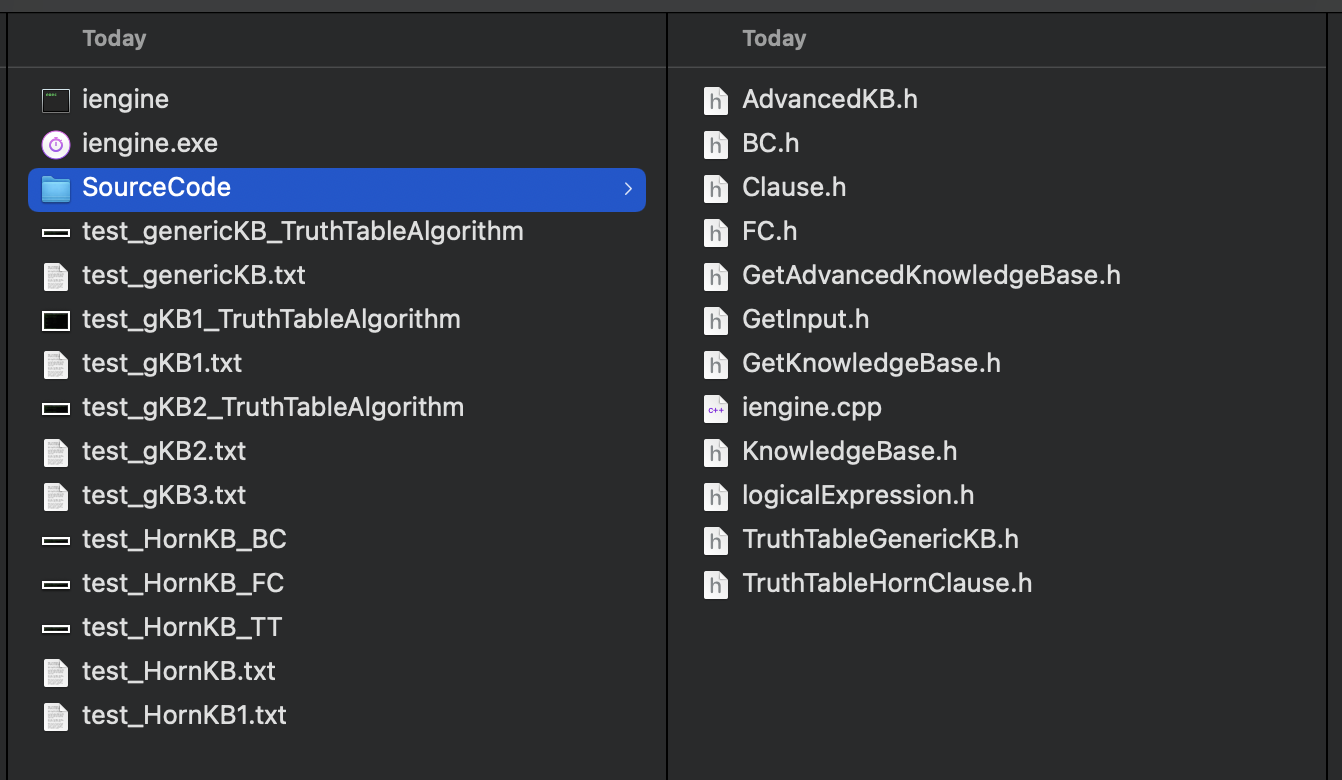
\includegraphics[width=0.7\textwidth]{./assets/FileOrganization.png}
    \caption{File Organization}
    \label{fig:fig1}
\end{figure}


\subsection{MacOS User}
For those who use MacOS systems, here is the command line to run the program on the terminal

\begin{verbatim}
Assignment2 % ./iengine FC test_HornKB.txt 
\end{verbatim}

The searching method \textbf{FC} can be replaced by \textbf{BC, TT} to deal with knowledge base containing only Horn Clauses.


To deal with generic knowledge, the method is \textbf{TTGeneric}:

\begin{verbatim}
Assignment2 % ./iengine TTGeneric test_genericKB.txt 
\end{verbatim}


\subsection{Microsoft Windows 11 User}
For those who use the Microsoft Windows Operating Systems, especially Windows 11, here is the command line to run the program in the \textbf{cmd}

\begin{verbatim}
PS D:\Desktop\Assignment2> ./iengine FC test_HornKB.txt 
\end{verbatim}

\begin{verbatim}
PS D:\Desktop\Assignment2> ./iengine TTGeneric test_genericKB.txt 
\end{verbatim}



\subsection{Input Requirements}
The program requires some requirements in order to execute.
\subsubsection{Horn Clause Knowledge Base}

\begin{itemize}
  \item Each symbol must be separated by a space
  \item The premise must not contain the bracket
  \item Every clause in the knowledge base should be followed by a semicolon
\end{itemize}

Here is a valid input for Horn Clause Knowledge Base: 
\begin{lstlisting}[caption={Valid Input For Horn Clause}]
TELL
p2 => p3; p3 => p1; c => e; b & e => f; f & g => h; p1 => d; p1 & p3 => c; a; b; p2;
ASK
d  
\end{lstlisting}

\subsubsection{Generic Knowledge Base}

For generic knowledge base, here are some requirements to be fulfilled:
\begin{itemize}
  \item Each symbol must be separated by a space
  \item It should contain the brackets allowing the program recognizes each logical expression precisely.
  \item Every clause in the knowledge base should be followed by a semicolon
\end{itemize}

Here is the demonstration of valid and invalid generic knowledge base:

\begin{lstlisting}[caption={Valid Input For Generic Knowledge Base}]
TELL
(a <=> (c => ~d)) & b & (b => a); c; ~f || g;
ASK
d
\end{lstlisting}

\begin{lstlisting}[caption={Invalid Input For Generic Knowledge Base}]
TELL
a <=> c => ~d & b & (b => a); c; ~f || g;
ASK
d
\end{lstlisting}



\section{Implementation For Horn Clause Knowledge Base Checking}

\subsection{Horn Clause}
A Horn Clause contains the premise and conclusion part. For example, here is a list of example of Horn Clause: $(A \land B) \Rightarrow C$, $(A \land B \land C) \Rightarrow D$, $E$.

It is easy to conclude that the premise contains a list of symbols and the conclusion is a symbol. For the Horn Clause as propositional symbol (eg. $E$), I will treat this expression as a clause with only conclusion. Figure \ref{fig:fig2} is my implementation in coding session.

\begin{figure}[h]
    \centering
    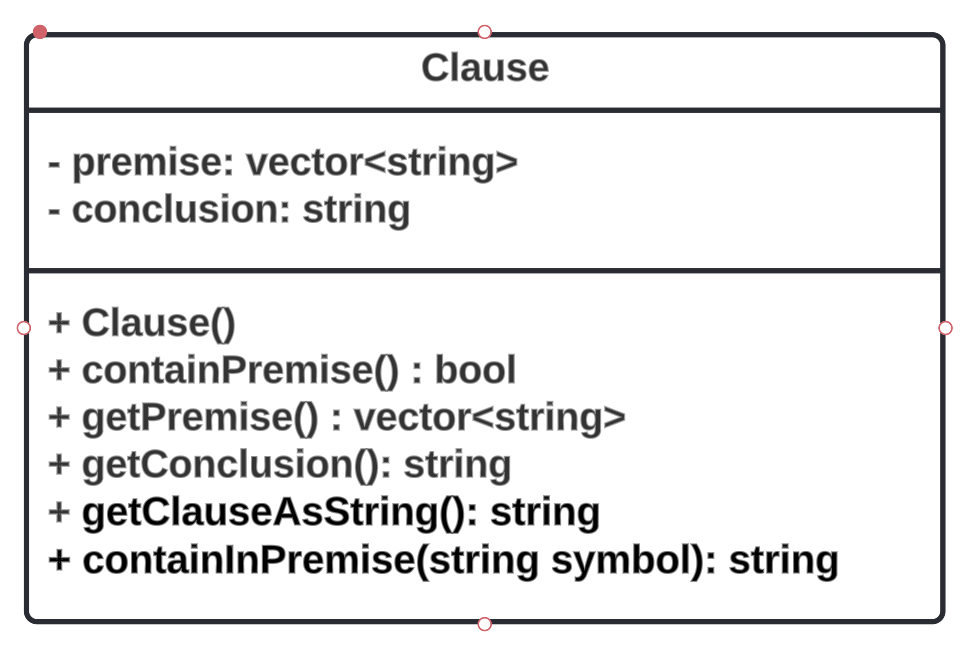
\includegraphics[width=0.4\textwidth]{./assets/Clause.png}
    \caption{Implementation of Clause in Programming}
    \label{fig:fig2}
\end{figure}

The Clause class has two attribute: a string of conclusion and a list of symbols in the premise.

\textbf{Function Explaination:}
\begin{itemize}
  \item \texttt{containPremise()}: this function will return true if the clause contains premise
  \item \texttt{getPremise()}: Function returns a list of symbols in the premise
  \item \texttt{getConclusion()}: Function returns the conclusion as a string
  \item \texttt{getClauseAsString()}: Function returns the entire clause as a string
\item \texttt{containedInPremise(string symbol)}: Function checks whether the given symbol is contained in the premise
  
\end{itemize}

\subsection{Knowledge Base}

A Knowledge Base simply contains a list of Horn Clause. Figure \ref{fig:fig3} is my implementation for knowledge base in programming.

\begin{figure}[h]
    \centering
    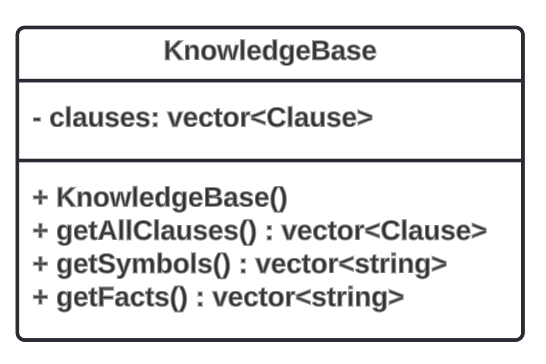
\includegraphics[width=0.4\textwidth]{./assets/KnowledgeBase.png}
    \caption{Implementation of Knowledge Base in Programming}
    \label{fig:fig3}
\end{figure}

The KnowledgeBase class has only one attribute: a list of Horn Clause

\textbf{Function Explaination:}
\begin{itemize}
  \item \texttt{getAllClauses()}: Function returns the list of Horn Clauses in the knowledge base
  \item \texttt{getSymbols()}: Function returns a list of symbols in the knowledge base.
  \item \texttt{getFacts()}: Function returns the list of propositional symbols. For example, given this knowledge base: $(A \land B) \Rightarrow C$, $(A \land B \land C) \Rightarrow D$, $E$, $M$ the function will return a list that contains $E$ and $M$. This function will be called by backward chaining algorithm.  
\end{itemize}

\subsection{Truth Table Checking}
The algorithm is provided in the lecture, so, this part does not include the theory. Instead, this section focus on my implementation. Figure 4 is an overview of the Truth Table Checking Agent.

\begin{figure}[h]
    \centering
    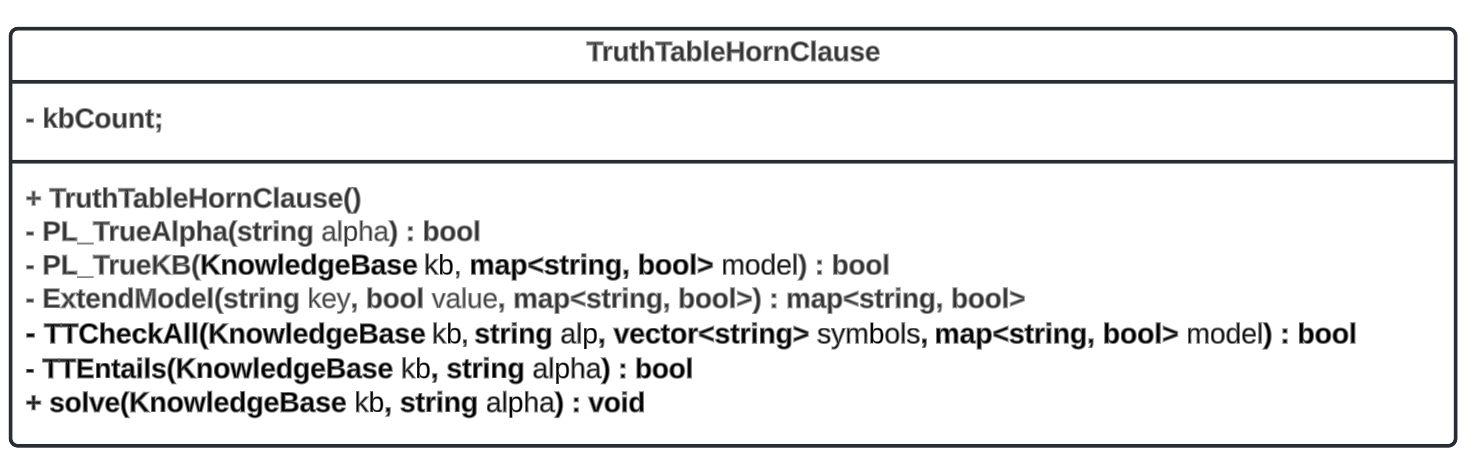
\includegraphics[width=0.9\textwidth]{./assets/TTHornClause.png}
    \caption{Implementation of Truth Table Checking in Programming}
    \label{fig:fig4}
\end{figure}

Given Knowledge Base and a query, we need to check whether the query can be entailed from Knowledge Base. By using Truth Table Checking, we will find all  models where KB is true, then if "for \textbf{ALL} models making our KB true, the value of the query is \textbf{always} true", we can conclude that the query can be entailed from the Knowledge Base.

To present a model, I used the data structure hash-map table \texttt{map<sring, bool>}, for example, supposed that here is our model: A true, B True, C False; then, this is the presented model (hash-map table) in coding: \texttt{model = \{'A': 1, 'B': 1, 'C': 0\}}.


\subsubsection{PLTrueAlpha() Function}

I will begin with the simplest function: \texttt{PLTrueAlpha()}. The function returns the value of the query in a given model.

\lstset{language=C++}
\begin{lstlisting}[caption={PLTrueAlpha() function}]
bool PL_TrueAlpha(string _query, map<string,bool> model){
     return model[_query];
}
\end{lstlisting}

\subsubsection{ExtendModel() Function}

This function takes a key, a value, and a current model, it adds a new pair key-value to that model, then it returns the new model with new key-value pair.

Here is my implementation code

\lstset{language=C++}
\begin{lstlisting}[caption={ExtendModel() function}]
map<string, bool> extendModel(string key, bool value, map<string, bool> &model){
    // Adding a new key-value pair using the insert() method
    model.insert(make_pair(key, value));
    return model;
}
\end{lstlisting}

\subsubsection{PLTrueKB() function}

This function will return True under one condition: with the given model, our KB is true. The lecture does not provide how to check the Horn Clause Knowledge base, so I would like to show my pseudocode. My implementation for this function can be found at the file \textbf{TruthTableHornClause.h}, in this report, I just provide my pseudocode for this function. 

\begin{algorithm}
\caption{PL\_TrueKB(knowledgeBase, model)}
\small % Set the font size to small
\begin{algorithmic}[1]
\Function{PL\_TrueKB}{knowledgeBase, model}
    \State $\text{listOfClause} \gets \text{getting from knowledgeBase}$
    \State $\text{output} \gets \text{True}$
    
    \For{$\text{clause in listOfClause}$}
        \State $\text{valueOfClauseWithThisModel} \gets \text{True}$
        
        \If{$\text{the clause contains only conclusion}$}
            \State $\text{valueOfClauseWithThisModel} \gets \text{model[conclusionOfClause]}$
        \Else
            \State $\text{listOfSymbolsInPremise} \gets \text{getting from clause}$
            \State $\text{conclusionOfClause} \gets \text{getting from clause}$
            
            \If{$\text{model[conclusionOfClause]}$ is True}
                \State $\text{valueOfClauseWithThisModel} \gets \text{True}$
            \Else
                \State $\text{conjunction} \gets \text{True}$
                \For{$\text{symbol in listOfSymbolsInPremise}$}
                    \State $\text{conjunction} \gets \text{conjunction \textbf{And} model[symbol]}$
                \EndFor
                
                \State $\text{valueOfClauseWithThisModel} \gets \text{valueOfClauseWithThisModel And !(conjunction)}$
            \EndIf
        \EndIf
        \State $\text{output} \gets \text{output \textbf{And} valueOfClauseWithThisModel}$
    \EndFor
    
    \State \Return $\text{output}$
\EndFunction
\end{algorithmic}
\end{algorithm}

This Idea is inspired by the fact $(A \rightarrow B)$ is equivalent to $(\lnot A \vee B)$

The algorithm traverses every clause in the knowledge base, if the clause is only a propositional symbol, then, the value of this clause is the value of the symbol in the model. Or else: if the clause contains premise and conclusion, we have 2 cases to be considered:

\begin{itemize}
  \item \textbf{Case 1:} if the value of the conclusion is true, then definitely the value of the clause is true.
  \item \textbf{Case 2:} if the value of the conclusion is false, we will get the conjunction of all symbols in the premise, if the conjunction value is false, the value of the clause is true.
\end{itemize}

Above is the explanation for pseudocode from lines 4-22.

In my coding, to get the list of clause from knowledge base (line 2 in the pseudocode above), I called the \texttt{getAllClauses()} function as below:

\lstset{language=C++}
\begin{lstlisting}[caption={Getting the list of clauses from Knowledge Base}]
vector<Clause> listOfClause = kb.getAllClauses();
\end{lstlisting}

In line 6, to check whether the current clause contains only conclusion, the program called the \textbf{containPremise()} from the \textbf{Clause} class as below:

\lstset{language=C++}
\begin{lstlisting}[caption={Coding for lines 6-7}]
if (currentClause.containPremise() == false){
     valueOfCurrentClauseWithThisModel = model[currentClause.getConclusion()];
}
\end{lstlisting}

To get the list of symbols in the premise and the conclusion of the clause, I used \texttt{getPremise()} method and \texttt{getConclusion()} method from the \textbf{Clause} class.

\subsubsection{TTCheckAll() Function}

My full implementation for this function can be found at at the file \textbf{TruthTableHornClause.h}, here is the pseudocode demonstrating my idea for this function.
                                                                                                                                                                                                                                                                                                                                                                                                                                                                                                                                                                                                                                                
                                                                                                                                                                                                                                                                                                                                                                                                                                                                                                                                                                                                                                              \begin{algorithm}
\caption{TT\_CheckAll(knowledgeBase, alpha, listOfSymbols, model)}
\small
\begin{algorithmic}[1]
\Function{TT\_CheckAll}{knowledgeBase, alpha, listOfSymbols, model}
    \If{$\text{listOfSymbols is Empty}$}
        \State Call PL\_TrueKB(knowledgeBase, model)
        \If{$\text{the output from PL\_TrueKB is True}$}
            \State Call PL\_TrueAlpha(alpha, model)
        \Else
            \State \Return True
        \EndIf
    \Else
        \State $P \gets \text{popping the first element from listOfSymbols}$
        
        \State $newModelWithPTrue \gets \text{Call ExtendModel(P, True, model)}$
        \State $newModelWithPFalse \gets \text{Call ExtendModel(P, False, model)}$
        
        \State \Return $\text{TT\_CheckAll(knowledgeBase, alpha, listOfSymbols, newModelWithPTrue)}$ \\
        \hspace{\algorithmicindent} $\text{\textbf{And} TT\_CheckAll(knowledgeBase, alpha, listOfSymbols, newModelWithPFalse)}$
    \EndIf
\EndFunction
\end{algorithmic}
\end{algorithm}

This algorithm is provided from the lecture, the \texttt{newModelWithPTrue} makes me confused at first, so I will show my implementation as below:

\lstset{language=C++}
\begin{lstlisting}[caption={Extend model}]
map<string, bool> restUnionWithPTrue = extendModel(P, true, model);
\end{lstlisting}

The \texttt{ExtendModel()} function will return a new model with the value of \textbf{P} and its boolean value, where:
\begin{itemize}
  \item \texttt{P} is the first element in the symbols list
  \item \texttt{model} is the model but without the value of \texttt{P}
\end{itemize}



                                                                                                                                                                                                                                                                                                                                                                                                                                                                                                                                                                                                                                               
                                                                                                                                                                                                                                                                                                                                                                                                                                                                                                                                                                                                                                               
                                                                                                                                                                                                                                                                                                                                                                                                                                                                                                                                                                                                                                               \subsubsection{TT\_Entail() Function and Solve() Function}
                                                                                                                                                                                                                                                                                                                                                                                                                                                                                                                                                                                                                                                                                                                                                                                                                                                                                                                                                                                                                                                                                                                                                                                                                                                                                          \texttt{TT\_Entails()} simply calls the \texttt{TT\_CheckAll()} and \texttt{Solve()} calls \texttt{TT\_Entails()}. So I will not discuss it right here.
                                                                                                                                                                                                                                                                                                                                                                                                                                                                                                                                                                                                                                                                                                                                                                                                                                                                                                                                                                                                                                                                                                                                                                                                                                                                                          \subsubsection{Result}
                                                                                                                                                                                                                                                                                                                                                                                                                                                                                                                                                                                                                                                                                                                                                                                                                                                                                                                                                                                                                                                                                                                                                                                                                                                                                         
                                                                                                                                                                                                                                                                                                                                                                                                                                                                                                                                                                                                                                                                                                                                                                                                                                                                                                                                                                                                                                                                                                                                                                                                                                                                                          
                                                                                                                                                                                                                                                                                                                                                                                                                                                                                                                                                                                                                                                                                                                                                                                                                                                                                                                                                                                                                                                                                                                                                                                                                                                                                          
                                                                                                                                                                                                                                                                                                                                                                                                                                                                                                                                                                                                                                                                                                                                                                                                                                                                                                                                                                                                                                                                                                                                                                                                                                                                       
                                                                                                                                                                                                                                                                                                                                                                                                                                                                                                                                                                                                                                                                                                                                                                                                                                                                                                                                                                                                                                                                                                                                                                                                                                                                                                                                                                                                                                                                                                                                                                                                                                                                                                                                                                                                                                                                                                                                                                                                                                                                                                                                                                                                                                                                                                                                                                                                                                                                                                                                                               
                                                                                                                                                                                                                                                                                                                                                                                                                                                                                                                                                                                                                                                                                                                                                                                                                                                                                                                                                                                                                                                                                                                                                                                                                                                                                                                                                                                                                                                                                                                                                                                                                                                                                                                                                                                                                                                                                                                                                                                                                                                                                                                                                                                                                                                                                                                                                                                                                                                                                                                                                                
                                                                                                                                                                                                                                                                                                                                                                                                                                                                                                                                                                                                                                                                                                                                                                                                                                                                                                                                                                                                                                                                                                                                                                                                                                                                                                                                                                                                                                                                                                                                                                                                                                                                                                                                                                                                                                                                                                                                                                                                                                                                                                                                                                                                                                                                                                                                                                                                                                                                                                                                                                 \begin{figure}[h]
    \centering
    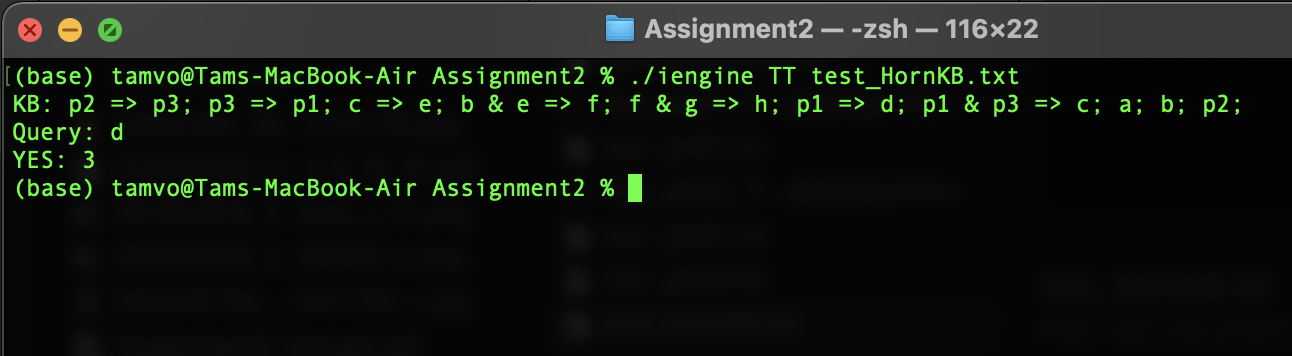
\includegraphics[width=0.8\textwidth]{./assets/resultTT.png}
    \caption{Result for Truth Table Checking Algorithm}
    \label{fig:fig4}
\end{figure}

\newpage
\subsection{Forward Chaining}

The pseudocode is provided in the lecture as Figure 6 below, this section will show my implementation for each line of pseudocodes.

\begin{figure}[h]
    \centering
    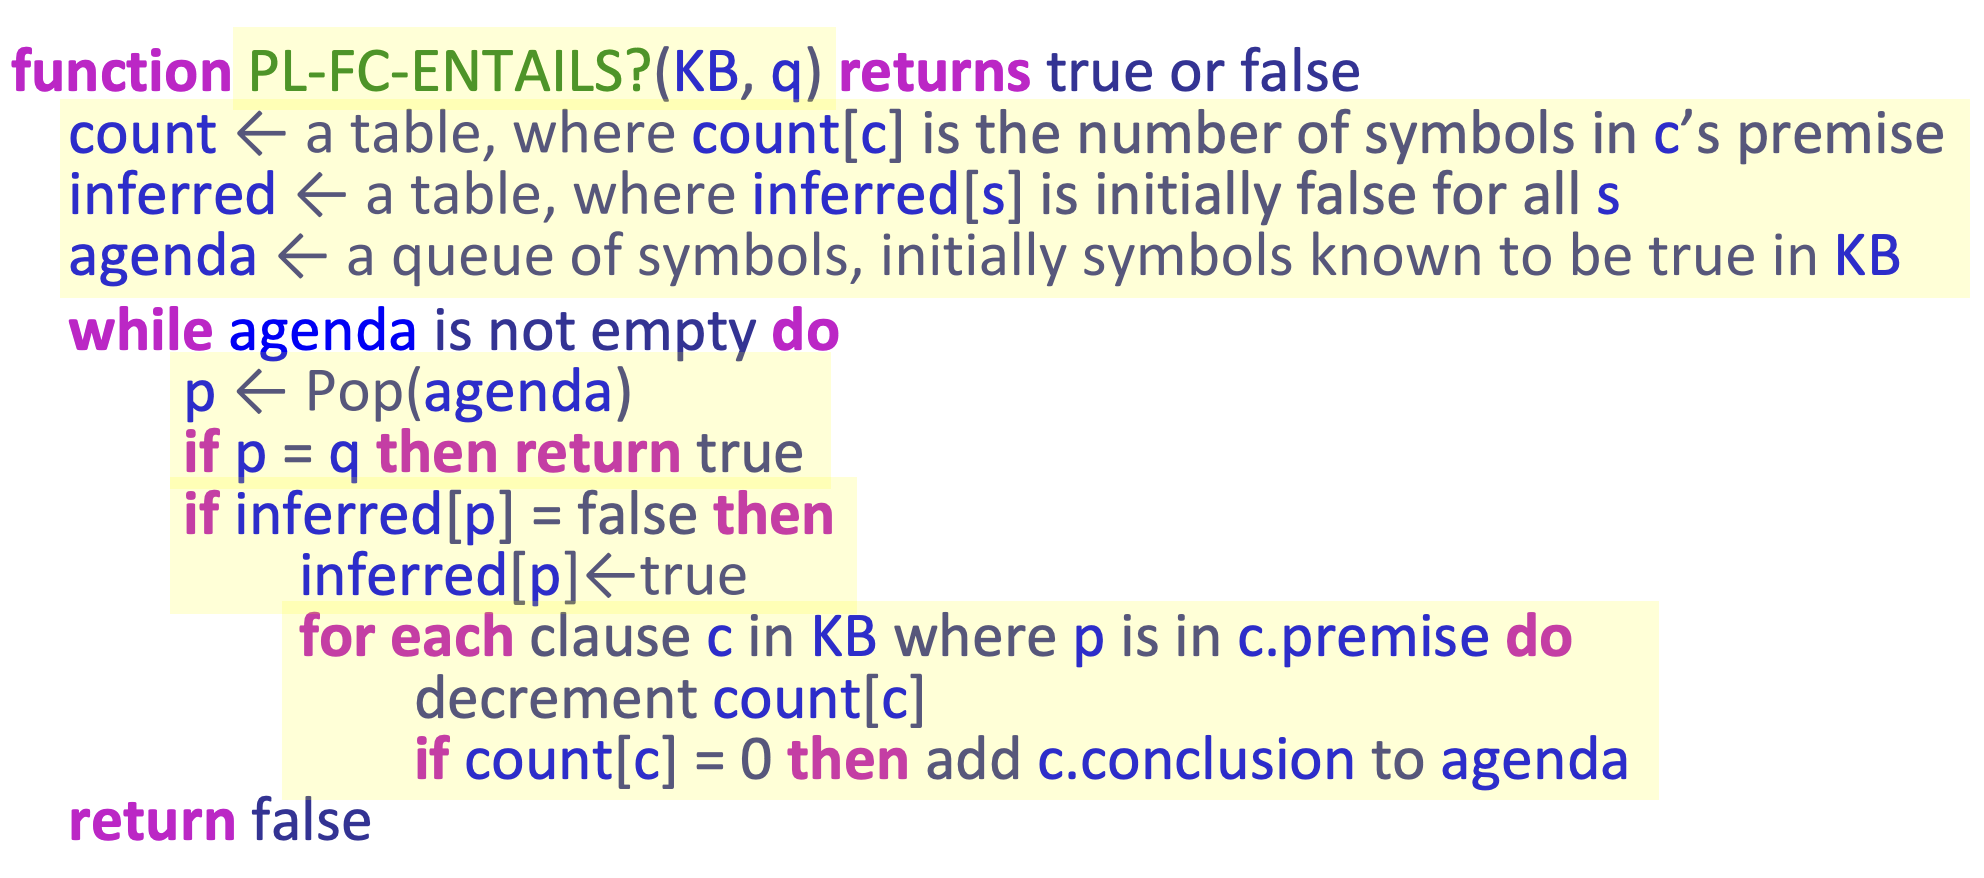
\includegraphics[width=0.8\textwidth]{./assets/FCpseu.png}
    \caption{Pseudocode for Forward Chaining Algorithm}
    \label{fig:fig5}
\end{figure}

\subsubsection{Count Table}

Again, I used the data structure hash-map table for this Count Table. The key is a string of propositional logic and the value is an integer.

\lstset{language=C++}
\begin{lstlisting}[caption={Define Count Table}]
	// define count
    map<string, int> count;
\end{lstlisting}

Then I traversed every clause and called the \texttt{getClauseAsString()} function to get the key for the clause. For the number of symbols in the premise, I called \texttt{getPremise()} function and count the number of element to get the value for this key:pair value.

\lstset{language=C++}
\begin{lstlisting}[caption={Initialize Count Table}]
for (int i = 0; i < listOfAllClause.size(); i++){
	Clause currentClause = listOfAllClause[i];
    string stringClause = currentClause.getClauseAsString();
    count.insert(make_pair(stringClause, currentClause.getPremise().size()));
}
\end{lstlisting}

\subsubsection{Inferred}

The \texttt{map<string, bool>} data structure is applied again. All I did is traversing the list taken from \textbf{Knowledge Base} function: \texttt{getSymbols()} and inserting key-value pair to inferred hash map table. 

\lstset{language=C++}
\begin{lstlisting}[caption={Define Inferred}]
    map<string, bool> inferred;
    // adding to inferred
     for (int i = 0; i < listOfAllSymbol.size(); i++){
         string currentSymbol = listOfAllSymbol[i];
         inferred.insert(make_pair(currentSymbol, false));
     }
\end{lstlisting}

\subsubsection{Agenda}
For Agenda, I applied the queue data structure as below:

\lstset{language=C++}
\begin{lstlisting}[caption={Define Agenda}]
	// define ageneda
    queue<string> agenda;
\end{lstlisting}

\subsubsection{Executing}

Here is my implementation in coding for the rest of the pseudocode:

\lstset{language=C++}
\begin{lstlisting}[caption={Checking the queue/agenda}]
	while (agenda.empty() == false){
          string currentSymbol = agenda.front();
          agenda.pop();
          propositionalSymbol.push(currentSymbol);

          if (currentSymbol == query){
               return true;
          }

          if (inferred[currentSymbol] == false){
               inferred[currentSymbol] = true;

            	// traverse every clause
                for (int i = 0; i < listOfAllClause.size(); i++){
                    Clause currentClause = listOfAllClause[i];

                    /// checking "currentSymbol" is in the premise of the current Clause or not
                    if (currentClause.containedInPremise(currentSymbol)){
                        count[currentClause.getClauseAsString()]--;
                        if (count[currentClause.getClauseAsString()] == 0){
                            agenda.push(currentClause.getConclusion());
                        }
                    } 
                }
           }
      }
            
      return false;
\end{lstlisting}
                                                                                                                                                                                                                                                                                                                                                                                                                                                                                                                                                                                                                                                                                                                                                                                                                                                                                                                                                                                                                                                                                                                                                                                                                                                                                                                                                                                                                                                                                                                                                                                                                                                                                                                                                                                                                                                                                                                                                                                                                                                                                                                                                                                                                                                                                                                                                                                                                                                                                                                                                                
                                                                                                                                                                                                                                                                                                                                                                                                                                                                                                                                                                                                                                                                                                                                                                                                                                                                                                                                                                                                                                                                                                                                                                                                                                                                                                                                                                                                                                                                                                                                                                                                                                                                                                                                                                                                                                                                                                                                                                                                                                                                                                                                                                                                                                                                                                                                                                                                                                                                                                                                                                \newpage
                                                                                                                                                                                                                                                                                                                                                                                                                                                                                                                                                                                                                                                                                                                                                                                                                                                                                                                                                                                                                                                                                                                                                                                                                                                                                                                                                                                                                                                                                                                                                                                                                                                                                                                                                                                                                                                                                                                                                                                                                                                                                                                                                                                                                                                                                                                                                                                                                                                                                                                                                                \subsubsection{Result}
                                                                                                                                                                                                                                                                                                                                                                                                                                                                                                                                                                                                                                                                                                                                                                                                                                                                                                                                                                                                                                                                                                                                                                                                                                                                                                                                                                                                                                                                                                                                                                                                                                                                                                                                                                                                                                                                                                                                                                                                                                                                                                                                                                                                                                                                                                                                                                                                                                                                                                                                                                
                                                                                                                                                                                                                                                                                                                                                                                                                                                                                                                                                                                                                                                                                                                                                                                                                                                                                                                                                                                                                                                                                                                                                                                                                                                                                                                                                                                                                                                                                                                                                                                                                                                                                                                                                                                                                                                                                                                                                                                                                                                                                                                                                                                                                                                                                                                                                                                                                                                                                                                                                             Here is some outputs using Forwarding Chaining Algorithm:
                                                                                                                                                                                                                                                                                                                                                                                                                                                                                                                                                                                                                                                                                                                                                                                                                                                                                                                                                                                                                                                                                                                                                                                                                                                                                                                                                                                                                                                                                                                                                                                                                                                                                                                                                                                                                                                                                                                                                                                                                                                                                                                                                                                                                                                                                                                                                                                                                                                                                                                                                             
                                                                                                                                                                                                                                                                                                                                                                                                                                                                                                                                                                                                                                                                                                                                                                                                                                                                                                                                                                                                                                                                                                                                                                                                                                                                                                                                                                                                                                                                                                                                                                                                                                                                                                                                                                                                                                                                                                                                                                                                                                                                                                                                                                                                                                                                                                                                                                                                                                                                                                                                                             \begin{figure}[h]
    \centering
    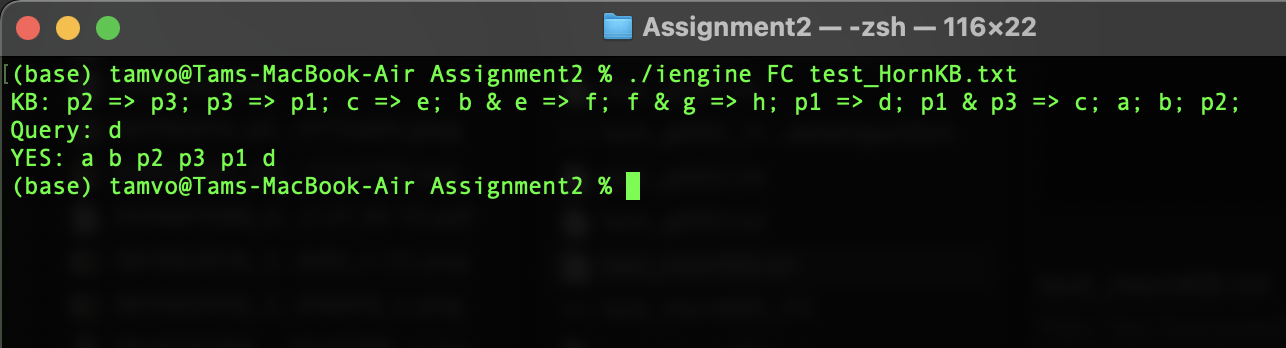
\includegraphics[width=0.9\textwidth]{./assets/test_HornKB_FC.png}
    \caption{Result 1}
    \label{fig:fig5}
\end{figure}

\begin{figure}[h]
    \centering
    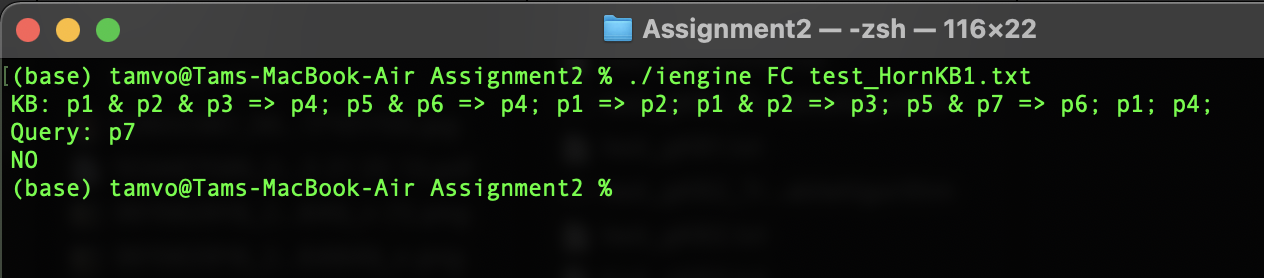
\includegraphics[width=0.9\textwidth]{./assets/test_HornKB1_FC.png}
    \caption{Result 2}
    \label{fig:fig6}
\end{figure}

\subsection{Backward Chaining}

The lecture does not provide the pseudocode of backward chaining algorithm, so I wil propose my pseudocode to solve the problem. The algorithm applied the recursion concept to find out the solution. You can find the coding implementation in the file \textbf{BC.h}.

The data structure hash-map is used again in backward chaining. But first we need to figure out what is fact in a given knowledge base. Supposed that we have this knowledge base: $(A \land B) \Rightarrow C$, $(A \land B \land C) \Rightarrow D$; $E$; $M$. We all know the "FACT" that $E$ and $M$ are always \textbf{True} in any models satisfying our Knowledge Base. That is, I will use a hash-map to store the Fact lists. In the given example, our fact list is \texttt{map<string, bool> fact = \{ 'E' : True, 'M' : True \}}. Here is my implementation:


\lstset{language=C++}
\begin{lstlisting}[caption={Define Fact}]
	map<string, bool> fact;	
	vector<string> factList = kb.getFact();
    for (int i = 0; i < factList.size(); i++){
        fact.insert(make_pair(factList[i], true));
    }
\end{lstlisting}

\newpage
\subsubsection{Proposed Algorithm}

\begin{algorithm}
\caption{BC\_Entail(knowledgeBase, query)}
\begin{algorithmic}[1]
\Function{BC\_Entail}{knowledgeBase, query}
   
    \If{$\text{query in fact}$}
        \State \Return True
    \EndIf
    
    \State $\text{listOfClauses} \gets \text{getting from knowledgeBase}$
    \State $\text{output} \gets \text{True}$
    
    \For{$\text{clause in listOfClauses}$}
        \If{$\text{query is a conclusion of clause}$}
   
            \State $\text{premiseList} \gets \text{getting from clause}$
            
            \For{$\text{symbol in premiseList}$}
                \State $\text{output} \gets \text{output \textbf{And} BC\_Entail(knowledgeBase, query)}$
                
                \If{$\text{output is True}$}
                    \State $\text{fact} \gets \text{insert new key:value (query: True)}$
                \EndIf
            \EndFor
        \EndIf
    \EndFor
    
    \State \Return $\text{fact[query]}$
\EndFunction
\end{algorithmic}
\end{algorithm}

\textbf{Explanation}

In this algorithm, we recursively check the premise until we reach the fact. Given this Knowledge Base: $A$; $B$; $(A \land B) \Rightarrow L$; $(A \land P) \Rightarrow L$; $(P \land L) \Rightarrow M$; $(L \land M) \Rightarrow P$; $P \Rightarrow Q$. We are interested in whether $Q$ can be entailed from KB, then we need to check whether $P$ can be proved. But to check whether $P$ can be proved, we need to check whether $L$ and $M$ can be proved, doing so until we reach our fact, which contains $A$ and $B$. By applying the concept of recursion, I solved this problem. 

In line 2, which is the base case of recursion, to check whether the fact contains the query, I used the built-in function by C++, here is my implementation:

\lstset{language=C++}
\begin{lstlisting}[caption={Checking whether fact contains query}]
if (fact.count(query) > 0){
   return true;
}
\end{lstlisting}

In line 5, to get the list of clauses from the knowledge base, I called the method \texttt{getAllClauses()} from \textbf{KnowledgeBase} class. This method is demonstrated before, so you can check again. Then, in line 8, to check whether the query is a conclusion of the given clause, I used the \texttt{getConclusion()} method as below:

\lstset{language=C++}
\begin{lstlisting}[caption={Checking whether the query is the conclusion of the given clause}]
if (currentClause.getConclusion() == query){
   ///coding
}
\end{lstlisting}

If the query is the conclusion of the current clause, then, in the conditional statement above, I created a list of symbols in the premise by calling the method \texttt{getPremise()} from the \textbf{Clause} class and recursively checked until I reached the fact as below:

\lstset{language=C++}
\begin{lstlisting}[caption={Implementation from lines 7 to 18}]
bool output = true;
            for (int i = 0; i < listOfClauses.size(); i++){
                Clause currentClause = listOfClauses[i];
                if (currentClause.getConclusion() == query){
                    
                    // traverse all symbols in the premise
                    vector<string> premiseList = currentClause.getPremise();
                    for (int j = 0; j < premiseList.size(); j++){
                        output = output && BC_Entail(kb, premiseList[j]);   
                        if (output){
                            fact.insert(make_pair(query, true));
                        }
                    }
                }
            }
            return fact[query];
\end{lstlisting}

\subsubsection{Result}
                                                                                                                                                                                                                                                                                                                                                                                                                                                                                                                                                                                                                                                                                                                                                                                                                                                                                                                                                                                                                                                                                                                                                                                                                                                                                                                                                                                                                                                                                                                                                                                                                                                                                                                                                                                                                                                                                                                                                                                                                                                                                                                                                                                                                                                                                                                                                                                                                                                                                                                                                            
                                                                                                                                                                                                                                                                                                                                                                                                                                                                                                                                                                                                                                                                                                                                                                                                                                                                                                                                                                                                                                                                                                                                                                                                                                                                                                                                                                                                                                                                                                                                                                                                                                                                                                                                                                                                                                                                                                                                                                                                                                                                                                                                                                                                                                                                                                                                                                                                                                                                                                                                                             
                                                                                                                                                                                                                                                                                                                                                                                                                                                                                                                                                                                                                                                                                                                                                                                                                                                                                                                                                                                                                                                                                                                                                                                                                                                                                                                                                                                                                                                                                                                                                                                                                                                                                                                                                                                                                                                                                                                                                                                                                                                                                                                                                                                                                                                                                                                                                                                                                                                                                                                                                            \begin{figure}[h]
    \centering
    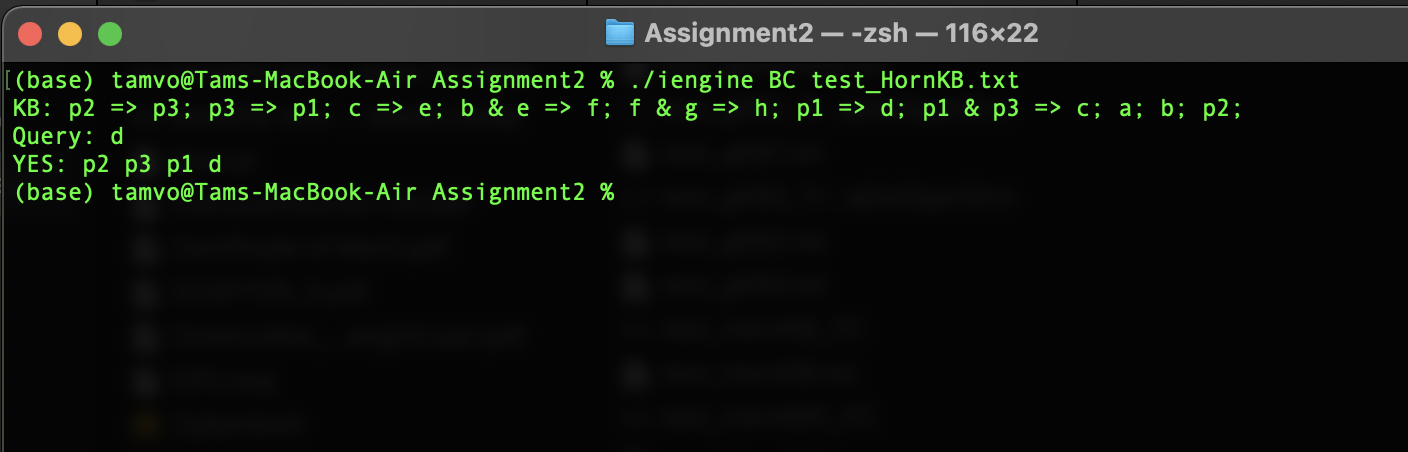
\includegraphics[width=0.8\textwidth]{./assets/test_HornKB_BC.png}
    \caption{Result 1}
    \label{fig:fig8}
\end{figure}

\begin{figure}[h]
    \centering
    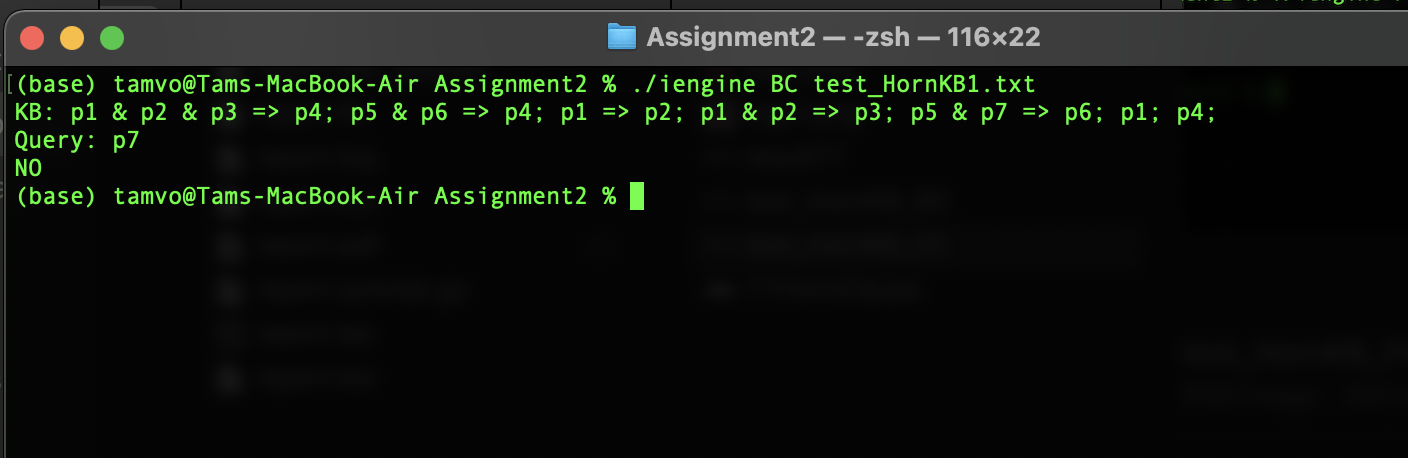
\includegraphics[width=0.8\textwidth]{./assets/test_HornKB1_BC.png}
    \caption{Result 2}
    \label{fig:fig10}
\end{figure}

\section{Research: Applying Recursion to Check Generic Knowledge Base}
\subsection{Problem Define}
The lecture provides algorithms: Truth Table Checking, Forward Chaining, Backward Chaining to check whether a propositional symbol can be entaiiled from a given knowledge base. However, these algorithms are used for the problem with Horn Clause, if the knowledge base is a general form, the problem can not be solved.

For example, given this knowledge base:

\[
(a \iff (c \Rightarrow \neg d)) \land b \land (b \Rightarrow a); c; \neg f \lor g;
\]

The question is whether $D$ can be entailed from the given Knowledge Base. As human being, we will generate all possible combination, there are 6 unique symbols, so there are $2^{6}=64$ models in total and check each model respectively. But for a model with 10 different symbols, it is impossible to traverse $2^10 = 1024$ models. This research will cover the explanation of a program checking whether a query can be entailed from a given generic knowledge base.

\subsection{Methodology and Implementation}

\subsubsection{Logical Expression Coding Presentation}
The atomic element in a knowledge base is a logical expression, for example, here is the list of logical expression: $(a \iff (c \Rightarrow \neg d))$, $a$, $(b \Rightarrow a)$, etc. Here is the implementation of class \textbf{logicalExpression}:

\begin{figure}[h]
    \centering
    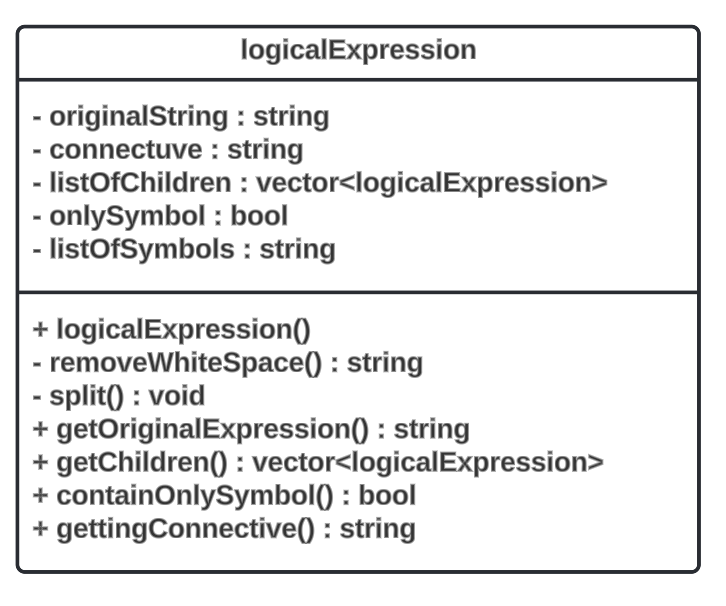
\includegraphics[width=0.4\textwidth]{./assets/logicalExpression.png}
    \caption{\textbf{logicalExpression} class in programming}
    \label{fig:fig11}
\end{figure}

The class has 5 attribute:

\begin{itemize}
	\item \texttt{originalString} is the logical expression as a string
	\item \texttt{connective} is the main connective of the logical expression (Eg. $\Rightarrow$, $\iff$, etc.)
	\item \texttt{listOfChildren} is a list of logical expression children (Eg. $(a \iff (c \Rightarrow \neg d))$ has 2 children, which are: $a$ and $(c \Rightarrow \neg d)$)
	\item \texttt{onlySymbol} is true if the current logical expression is a propositional symbol
	\item \texttt{listOfSymbols} is a list that contains all symbols in the logical expression
\end{itemize}

\textbf{Function explanation}

\begin{itemize}
	\item \texttt{split()} functions finds the children and connective of current logical expression, then adds logical expression child to \texttt{listOfChildren}
	\item \texttt{getOriginalExpression()} function returns the logical expression as a string.
	\item \texttt{getChildren()} function returns \texttt{listOfChildren}
	\item \texttt{containOnlySymbol()} function returns true if the the logical expression is a propositional symbol
	\item \texttt{gettingConnective()} function returns the main connective of the logical expression
\end{itemize}

For example, the expression $(a \iff (c \Rightarrow \neg d))$ has these properties: 

\begin{itemize}
\item \texttt{originalString} is $(a \iff (c \Rightarrow \neg d))$
	\item \texttt{connective} is $\iff$
	\item \texttt{listOfChildren} contains $a$ and $(c \Rightarrow \neg d)$. Both of them are logicalExpression datatype
	\item \texttt{onlySymbol} is \texttt{False}
	\item \texttt{listOfSymbols} is a list that contains: a, c, d
\end{itemize}

\subsubsection{Advanced Knowledge Base}
Advanced knowledge base contains a list of logical expressions and a function to return all symbols in the knowledge base.

\begin{figure}[h]
    \centering
    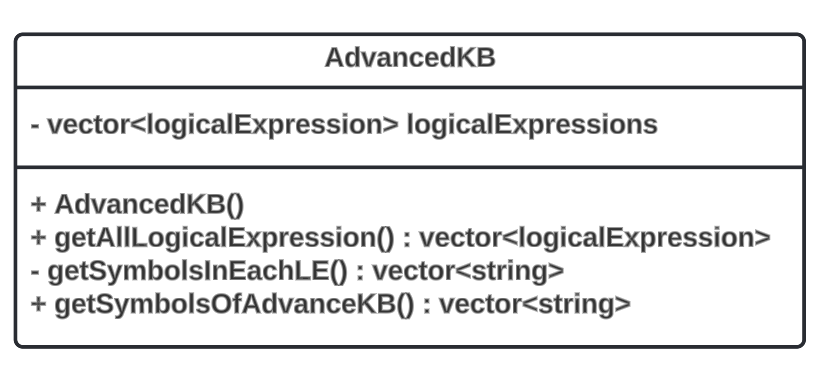
\includegraphics[width=1\textwidth]{./assets/AdvancedKB.png}
    \caption{\textbf{AdvancedKB} class in programming}
    \label{fig:fig13}
\end{figure}

\newpage
This section will discuss how to get every symbol in the knowledge base, but first, the pseudocode to get all symbol in a logical expression will be shown:

\begin{algorithm}
\caption{\texttt{getSymbolsInEachLE()} getting all symbols in a logical expression}
\begin{algorithmic}[1]
\Function{getSymbolsInEachLE}{logicalExpression}
    \State $output \gets \emptyset$
    
    \If{$\text{logicalExpression is a propositional symbol}$}
        \State $\text{Add logicalExpression to output}$
        \State \Return $output$
    \EndIf
    
    \For{$\text{child in logicalExpression}$}
        \State $\text{listOfSymbols} \gets \text{getSymbolsInEachLE(child)}$
        
        \For{$\text{symbol in listOfSymbols}$}
            \If{$\text{symbol not in output}$}
                \State $\text{add symbol to output}$
            \EndIf
        \EndFor
    \EndFor
    
    \State \Return $output$
\EndFunction
\end{algorithmic}
\end{algorithm}

For lines 3-5, the method \texttt{containOnlySymbol()} and \texttt{getOriginalExpression()} in the \textbf{logicalExpression} class will be called as below:

\lstset{language=C++}
\begin{lstlisting}[caption={Coding for lines 3-5}]
if (_logicalExpression.containOnlySymbol()){
    output.push_back(_logicalExpression.getOriginalExpression());
    return output;
}
\end{lstlisting}

Then, the algorithm will traverse every child of the logical expression and recursively called the \texttt{getSymbolsInEachLE()} until reaching the base case: the logical expression is a propositional symbol.

Here is the coding implementation:
\lstset{language=C++}
\begin{lstlisting}[caption={Coding for lines 7-15}]
for (int i = 0; i < _logicalExpression.getChildren().size(); i++){
     logicalExpression currentChild = _logicalExpression.getChildren()[i];
     vector<string> temp = getSymbolsInEachLE(currentChild);

     for (int j = 0; j < temp.size(); j++){
            
          // ensure the result is already in the output
          if (count(output.begin(), output.end(), temp[j]) == 0){
               output.push_back(temp[j]);
          }
      }
}
return output;
\end{lstlisting}

The method \texttt{getSymbolsOfAdvancedKB()} will traverse every logical expression in the knowledge base and call the \textbf{getSymbolsInEachLE()} method to extract a list of symbols.

\subsubsection{Truth Table Checking for generic knowledge base}

The algorithm will be the same as Truth Table Checking for Horn Clause. However, the function \texttt{PL\_TrueKB()} is different and there will be a another function handling the task model checking. Below is the pseudocode for \texttt{LogicalExpressionChecking()} function:

\begin{algorithm}
\caption{LogicalExpressionChecking(expression, model)}
\small
\begin{algorithmic}[1]
\Function{LogicalExpressionChecking}{expression, model}
    \If{$\text{logicalExpression is a propositional symbol}$}
        \State \Return $\text{model[logicalExpression]}$
    \EndIf
    
    \State $\text{listOfChildren} \gets \text{getting from logicalExpression}$
    \State $\text{connective} \gets \text{getting from logicalExpression}$
    
    \If{$\text{listOfChildren has 2 children}$}
        \State $\text{leftChild} \gets \text{listOfChildren[0]}$
        \State $\text{rightChild} \gets \text{listOfChildren[1]}$
        \State $\text{valueOfLeftChild} \gets \text{LogicalExpressionChecking(leftChild, model)}$
        \State $\text{valueOfRightChild} \gets \text{LogicalExpressionChecking(rightChild, model)}$
        
        \If{$\text{connective is \textbf{biconditional}}$}
            \If{$\text{valueOfLeftChild is True and valueOfRightChild is True}$}
                \State \Return $\text{True}$
            \ElsIf{$\text{valueOfLeftChild is False \textbf{And} valueOfRightChild is False}$}
                \State \Return $\text{True}$
            \EndIf
            
            \State \Return $\text{False}$
        \ElsIf{$\text{connective is \textbf{implication}}$}
            \State \Return $\text{\textbf{not} valueOfLeftChild \textbf{Or} valueOfRightChild}$
        \ElsIf{$\text{connective is disjunction}$}
            \State \Return $\text{valueOfLeftChild \textbf{Or} valueOfRightChild}$
        \ElsIf{$\text{connective is conjunction}$}
            \State \Return $\text{valueOfLeftChild \textbf{And} valueOfRightChild}$
        \EndIf
    \Else
        \State \Return $\text{\textbf{not} LogicalExpressionChecking(listOfChildren[0], model)}$
    \EndIf
\EndFunction
\end{algorithmic}
\end{algorithm}

The coding implementation can be found in the file \textbf{TruthTableGenericKB.h}. Look at the algorithm, there is a question: Why does a logical expression have 2 children? To answer this question, if there is a connective in the given expression, my implementation will consider 2 cases:

\begin{itemize}
\item the connective is \textbf{negation}: the whole part after the negation sign is the only child of the original expression
\item the connective is \textbf{biconditional}, \textbf{implication}, \textbf{conjunction}, \textbf{disjunction}: there are always 2 children. The first child is the expression before the connective, the second child is the expression after the connective.
\end{itemize}

For example, given this logical expression: \( (a \Rightarrow b) \land b \land (c \iff \neg d) \), the given logical expression has these properties:

\begin{itemize}
\item First Child: $(a \Rightarrow b)$
\item Second Child: $b \land (c \iff \neg d)$
\item Connective: Conjunction
\end{itemize}


Then the function \texttt{PL\_TrueKB(advancedKB, model)} will traverse every clause in the knowledge base and call the \texttt{LogicalExpressionChecking()} function. 

\begin{algorithm}
\caption{PL\_TrueKB(advancedKB, model)}
\small
\begin{algorithmic}[1]
\Function{PL\_TrueKB}{advancedKB, model}
    \State $\text{listOfLogicalExpression} \gets \text{getting from advancedKB}$
    \State $\text{output} \gets \text{True}$
    
    \For{$\text{expression in listOfLogicalExpression}$}
        \State $\text{valueOfExpression} \gets \text{Call LogicalExpressionChecking(expression, model)}$
        
        \State $\text{output} \gets \text{output And valueOfExpression}$
    \EndFor
    
    \State \Return $\text{output}$
\EndFunction
\end{algorithmic}
\end{algorithm}

\subsubsection{Result}
 Here are some results after applying my algorithm:
 
 \begin{figure}[h]
    \centering
    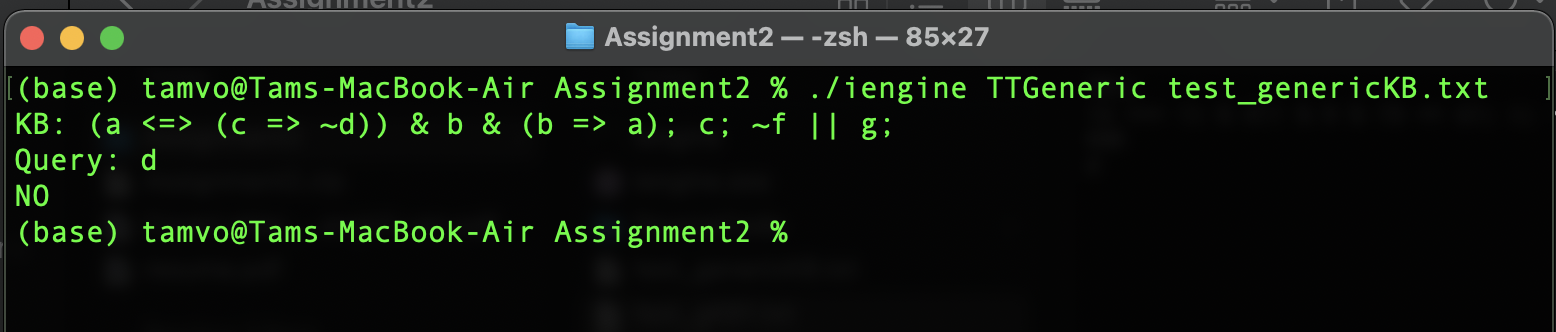
\includegraphics[width=0.7\textwidth]{./assets/test_genericKB_TruthTableAlgorithm.png}
    \caption{Result 1}
    \label{fig:fig99}
\end{figure}
 
  \begin{figure}[h]
    \centering
    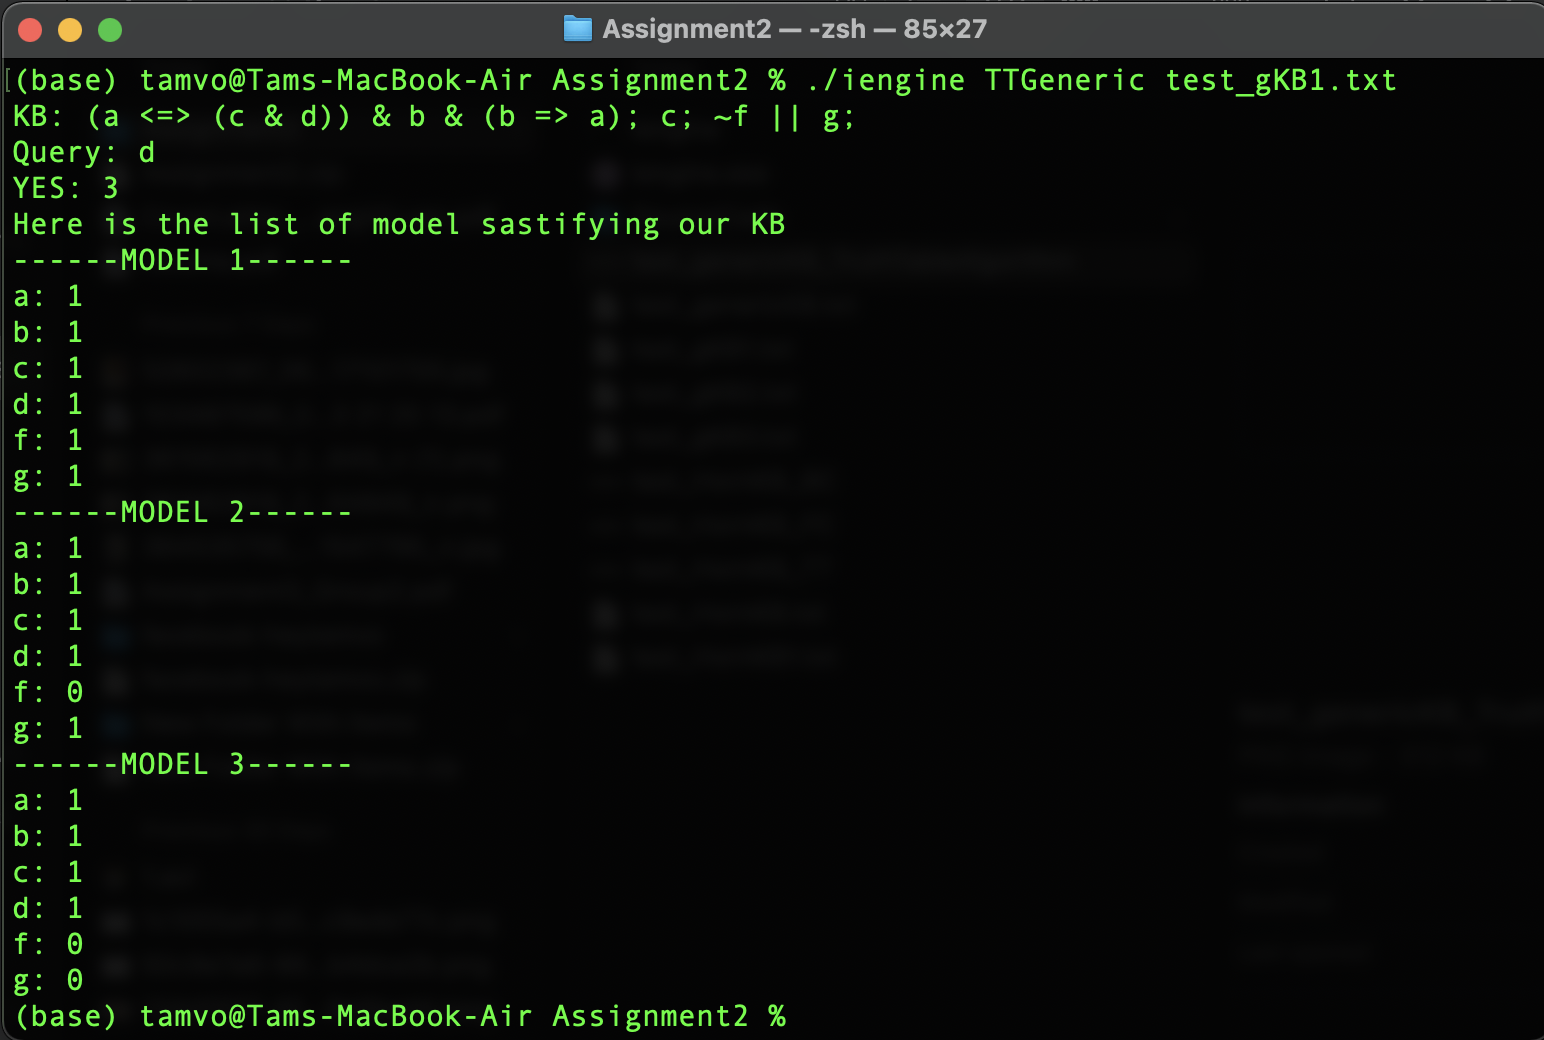
\includegraphics[width=0.6\textwidth]{./assets/test_gKB1_TruthTableAlgorithm.png}
    \caption{Result 2}
    \label{fig:fig999}
\end{figure}

 
 
 



                                                                                                                                                                                                                                                                                                                                                                                                                                                                                                                                                                                                                                                                                                                                                                                                                                                                                                                                                                                                                                                                                                                                                                                                                                                                                                                                                                                                                                                                                                                                                                                                                                                                                                                                                                                                                                                                                                                                                                                                                                                                                                                                                                                                                                                                                                                                                                                                                                                                                                                                                            

                                                                                                                                                                                                                                                                                                                                                                                                                                                                                                                                                                                                                                                                                                                                                                                                                                                                                                                                                                                                                                                                                                                                                                                                                                                                                                                                                                                                                                                                                                                                                                                                                                                                                                                                                                                                                                                                                                                                                                                                                                                                                                                                                                                                                                                                                                                                                                                                                                                                                                                                                              

                                                                                                                                                                                                                                                                                                                                                                                                                                                                                                                                                                                                                                                                                                                                                                                                                                                                                                                                                                                                                                                                                                                                                                                                                                                                                                                                                                                                                                                                                                                                                                                                                                                                                                                                                                                                                                                                                                                                                                                                                                                                                                                                                                                                                                                                                                                                                                                                                                                                                                                                                                         
                                                                                                                                                                                                                                                                                                                                                                                                                                                                                                                                                                                                                                                                                                                                                                                                                                                                                                                                                                                                                                                                                                                                                                                                                                                                                 
                                                                                                                                                                                                                                                                                                                                                                                                                                                                                                                                                                                                                                                                                                                                                                                                                                                                                                                                                                                                                                                                                                                                                                                                                                                                                 
                                                                                                                                                                                                                                                                                                                                                                                                                                                                                                                                                                                                                                                                                                                                                                                                                                                                                                                                                                                                                                                                                                                                                                                                                                                                                 
                                                                                                                                                                                                                                                                                                                                                                                                                                                                                                                                                                                                                                               
                                                                                                                                                                                                                                                                                                                                                                                                                                                                                                                                                                                                                                               




\end{document}

